\documentclass[]{article}

\usepackage{graphicx} 			% Imagens
\usepackage{amsmath}			% Matemático
\usepackage{amsfonts}			% Fontes
\usepackage[utf8]{inputenc}		% Acentos
\usepackage{float}				% Incluir figura no minipage
\usepackage[landscape]{geometry} % Modo paisagem
\usepackage{lscape}				 % Modo paisagem em uma seção
\usepackage{multicol}			 % Multicolunas


%opening
\title{Trabalhando com Alinhamentos}
\author{Lucas Arantes Berg}

\begin{document}

\maketitle

\begin{abstract}
	Aqui vai o resumo.
\end{abstract}

\section{Teste de Alinhamento}

\mbox{Texto não será separado.}

\fbox{Texto não se separa e possui uma caixa desenhada em seu entorno.}

\begin{minipage}{\linewidth}
	\centering
	\begin{minipage}{0.45\linewidth}
		Texto.
	\end{minipage}
	\hspace{0.05\linewidth}
	\begin{minipage}{0.45\linewidth}
		\begin{figure}[H]
			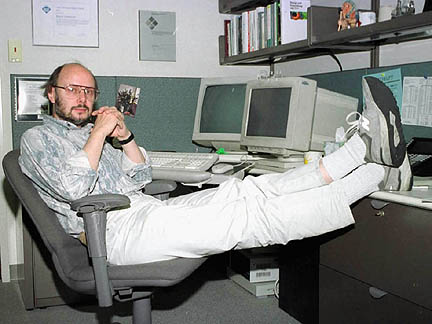
\includegraphics[width=\linewidth]{img/BjarneStroustrup.jpg}
			\caption{Bjarne Stroustrup, creator of C$++$.}
		\end{figure}
	\end{minipage}
\end{minipage}

\newpage
% Modo paisagem
\begin{landscape}
	\begin{table}
		\caption{Exemplo}
		\centering
		\begin{tabular}{lccc}
			\hline
			A & B & A & B \\
			\hline
			A & B & A & B \\
			C & D & C & D \\
			C & D & C & D \\
			\hline
		\end{tabular}
	\end{table}
\end{landscape}

% Multicolunas
\begin{multicols}{3}
	Texto contido dentro desse ambiente será exibido em duas colunas. O LATEX faza divisão das colunas
\end{multicols}

\end{document}
